\documentclass[conference]{IEEEtran}
\IEEEoverridecommandlockouts
\usepackage{cite}
\usepackage{amsmath,amssymb,amsfonts}
\usepackage{graphicx}
\usepackage{textcomp}
\usepackage{xcolor}
\usepackage{booktabs}
\usepackage{float}
\graphicspath{{screenshots/}}
\def\BibTeX{{\rm B\kern-.05em{\sc i\kern-.025em b}\kern-.08em
    T\kern-.1667em\lower.7ex\hbox{E}\kern-.125emX}}
\begin{document}

\title{Interactive Statistical Analysis of Personal Running Data Using Strava Exports}

\author{
\IEEEauthorblockN{Gian Federspiel}
\IEEEauthorblockA{
    \textit{Informatik}\\
    \textit{HSLU Lucerne University of Applied Sciences and Arts}\\
    Rotkreuz, Switzerland\\
    gian.federspiel@stud.hslu.ch}
\and
\IEEEauthorblockN{Seedorf Asamoah}
\IEEEauthorblockA{
    \textit{Informatik}\\
    \textit{HSLU Lucerne University of Applied Sciences and Arts}\\
    Rotkreuz, Switzerland\\
    seedorf.asamoah@stud.hslu.ch}
}

\maketitle

\begin{abstract}
This project presents an interactive web dashboard for the statistical analysis of personal running data exported from the Strava fitness platform. Users upload their own activity CSV file, which the application cleans and filters to running activities. The dashboard computes descriptive statistics and applies inferential methods including Pearson correlation and ordinary least squares linear regression to quantify pace trends over time and the relationship between heart rate and running pace. All results are visualised interactively using Plotly charts embedded in a Streamlit application.
\end{abstract}

\begin{IEEEkeywords}
running statistics, Strava, linear regression, Pearson correlation, Streamlit, data visualisation
\end{IEEEkeywords}

\section{Introduction}

Recreational running has become increasingly popular, and modern fitness trackers such as Strava record rich per-activity data including distance, moving time, and heart rate. While Strava itself provides aggregate summaries, it does not expose the underlying statistical relationships in a user-controllable way. This project fills that gap by providing an open-source dashboard that allows any Strava user to upload their own data export and immediately obtain statistically grounded insights about their training.

The primary research questions addressed by the dashboard are:
\begin{itemize}
    \item Has the athlete's running pace improved over time, and is the trend statistically significant?
    \item Is there a statistically significant linear relationship between average heart rate and running pace?
\end{itemize}

\section{Data}

\subsection{Source and Format}

Data is obtained via Strava's built-in export feature (Settings $\rightarrow$ My Account $\rightarrow$ Download or Delete Your Account $\rightarrow$ Request Your Archive). The downloaded archive contains an \texttt{activities.csv} file with one row per recorded activity and columns including activity date, type, distance, moving time, average heart rate, and elevation gain.

\subsection{Preprocessing}

The data processing pipeline (implemented in \texttt{data\_processor.py}) performs the following steps:

\begin{enumerate}
    \item \textbf{Column normalisation:} Column names are lower-cased and mapped to a consistent internal schema to handle differences between Strava export versions.
    \item \textbf{Activity filtering:} Only activities of type \textit{Run} or \textit{VirtualRun} are retained.
    \item \textbf{Unit conversion:} Distance values stored in metres (median $> 200$) are converted to kilometres. Moving time strings in \texttt{H:MM:SS} or \texttt{M:SS} format are parsed to seconds.
    \item \textbf{Pace computation:} Running pace (min/km) is derived as $\text{pace} = \frac{\text{moving time [min]}}{\text{distance [km]}}$. Implausible values outside $[3, 15]$ min/km are set to missing.
    \item \textbf{Temporal features:} ISO week start and calendar month start columns are added for aggregation.
\end{enumerate}

\section{Statistical Methods}

\subsection{Descriptive Statistics}

The dashboard reports the total number of runs, cumulative distance, mean pace, best (minimum) pace, longest single run, and mean heart rate across all runs. Rolling averages are computed over a window of 10 runs for pace and 8 runs for heart rate, providing a smoothed view of the athlete's training trajectory without being overly sensitive to individual outlier sessions.

\subsection{Weekly Volume}

Weekly running volume is computed by summing distances within each ISO calendar week and displayed as a bar chart, giving an immediate impression of training consistency and load distribution.

\subsection{Heart Rate Analysis}

For runs that include heart rate data, the dashboard provides two complementary views. First, a histogram with 25 bins shows the distribution of average heart rate across all runs, along with summary statistics (mean, minimum, maximum, and standard deviation). Second, a scatter plot with an 8-run rolling average shows how heart rate evolves over time — a downward trend at the same pace would indicate improved aerobic fitness.

\begin{figure}[H]
\centerline{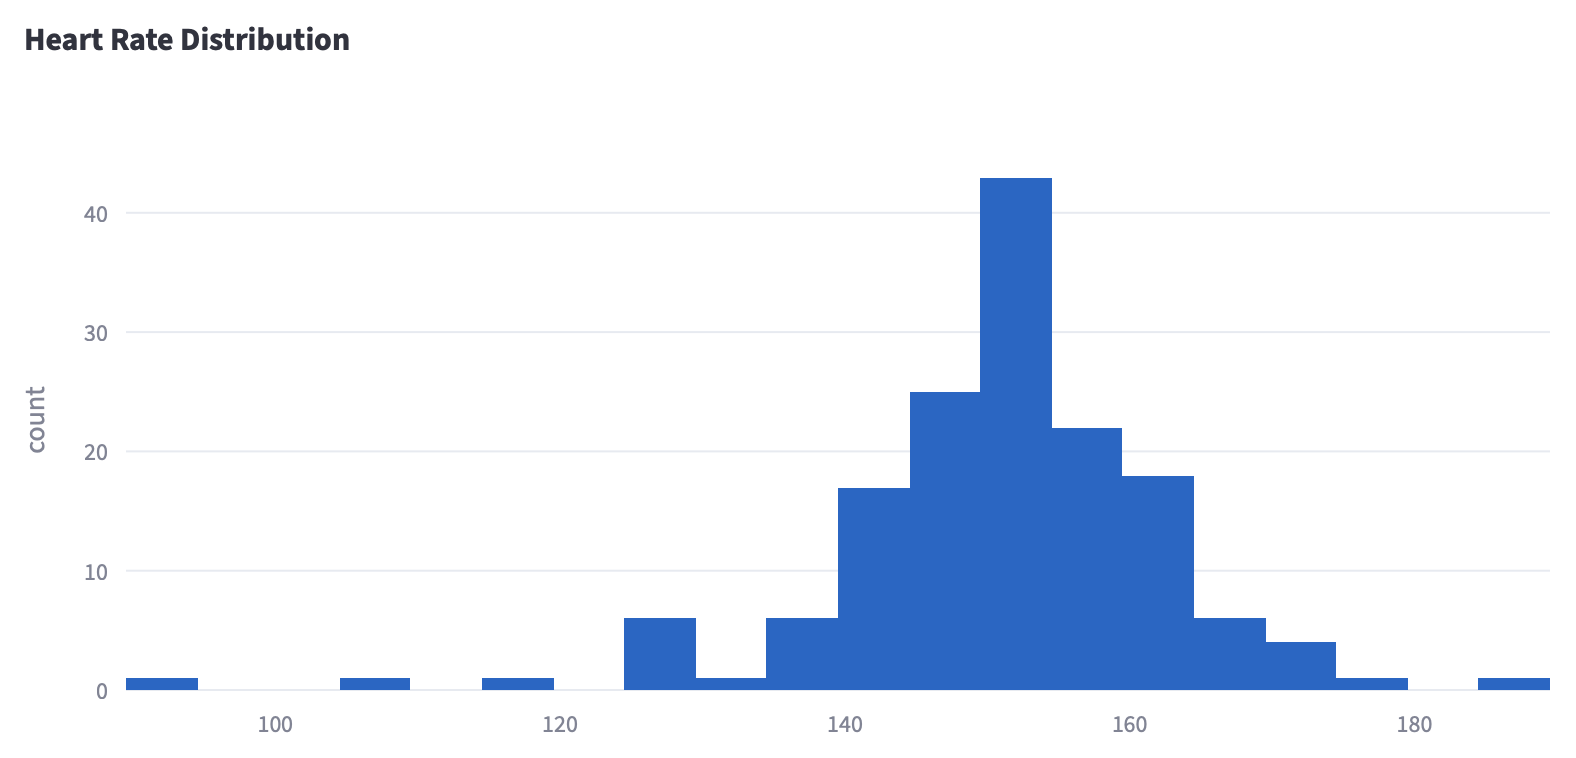
\includegraphics[width=\columnwidth]{heart_rate_distribution_screenshot.png}}
\caption{Heart rate distribution across all recorded runs. The distribution is roughly unimodal and right-skewed, with the majority of runs falling between 140 and 170 bpm and a clear peak around 150--155 bpm.}
\label{fig:hr_dist}
\end{figure}

\subsection{Pearson Correlation: Pace vs Heart Rate}

To quantify the relationship between cardiovascular load and running speed, the Pearson correlation coefficient $r$ is computed between average heart rate (bpm) and pace (min/km) across all runs with heart rate data:

\begin{equation}
    r = \frac{\sum (x_i - \bar{x})(y_i - \bar{y})}{\sqrt{\sum (x_i - \bar{x})^2 \sum (y_i - \bar{y})^2}}
\end{equation}

A two-sided $t$-test is applied to assess significance at $\alpha = 0.05$. The scatter plot includes an OLS trendline, and the dashboard reports $r$, $R^2$, $p$, and a plain-language interpretation of the direction (e.g.\ \textit{higher HR $\rightarrow$ slower pace}). Fig.~\ref{fig:hr_dist} shows the heart rate distribution from the example dataset. Fig.~\ref{fig:regression} shows the corresponding pace regression.

\subsection{Linear Regression: Pace Improvement over Time}

To test whether pace improves over the course of the athlete's recorded history, simple linear regression is fitted with sequential run number as the predictor and pace (min/km) as the response:

\begin{equation}
    \hat{y}_i = \beta_0 + \beta_1 \cdot i
\end{equation}

where $i$ is the run index (1-based). The slope $\beta_1$ expresses the average pace change per run. Combined with the observed run frequency, a monthly pace change is derived. Statistical significance is assessed at $\alpha = 0.05$ via the $F$-test $p$-value. All regression computations use \texttt{scipy.stats.linregress} \cite{scipy}.

\begin{figure}[H]
\centerline{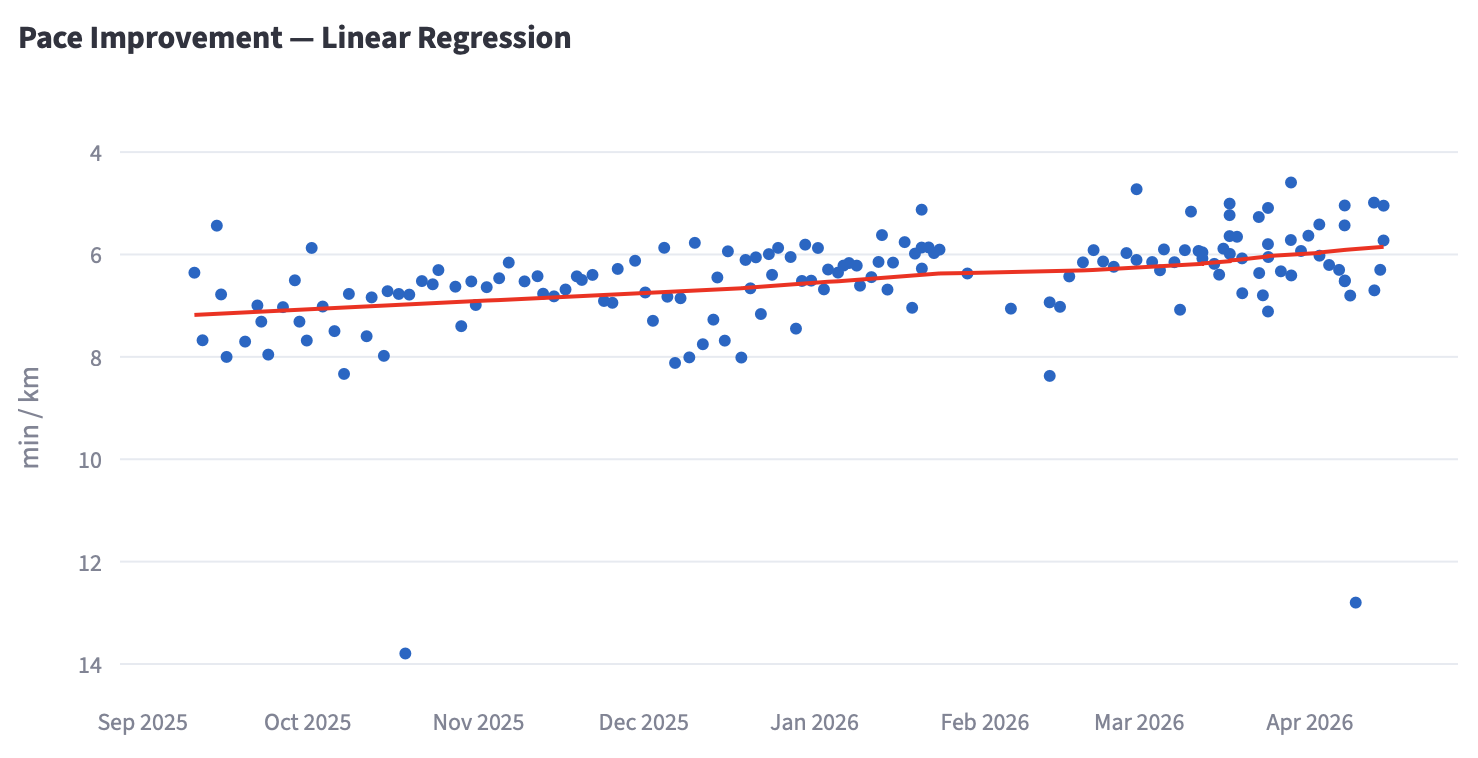
\includegraphics[width=\columnwidth]{linear_regression_screenshot.png}}
\caption{Pace improvement over time (Sep 2025 -- Apr 2026). Each point represents one run; the red line is the OLS regression fit. The upward visual trend corresponds to improving pace, as the y-axis is inverted (lower min/km = faster).}
\label{fig:regression}
\end{figure}

\section{Implementation}

The application is built in Python 3 using Pandas \cite{pandas} for data manipulation, SciPy \cite{scipy} for statistical computations, Plotly Express \cite{plotly} for interactive charts, and Streamlit \cite{streamlit} for the web interface. The codebase is split into \texttt{data\_processor.py} (ingestion and feature engineering) and \texttt{app.py} (layout and visualisation). Data is processed in memory and stored in Streamlit session state — nothing is written to disk or sent to external servers.

\section{Discussion and Conclusion}

The dashboard demonstrates that meaningful statistical analysis of personal fitness data is achievable with a concise, well-structured codebase. The combination of rolling averages, correlation analysis, and linear regression gives athletes an evidence-based view of their progress beyond simple cumulative totals.

A key limitation is that both models are univariate and do not control for confounders such as terrain or weather. Future work could incorporate multiple regression to address this, and direct OAuth integration with the Strava API would remove the manual export step.

Despite these limitations, the project achieves its goal of making statistical running analysis accessible to any Strava user through an intuitive, privacy-respecting, browser-based interface.

\begin{thebibliography}{00}
\bibitem{scipy} P. Virtanen et al., ``SciPy 1.0: Fundamental algorithms for scientific computing in Python,'' \textit{Nature Methods}, vol. 17, pp. 261--272, 2020.
\bibitem{pandas} W. McKinney, ``Data structures for statistical computing in Python,'' \textit{Proc. 9th Python in Science Conf.}, pp. 56--61, 2010.
\bibitem{streamlit} Streamlit Inc., ``Streamlit --- A faster way to build and share data apps,'' 2024. [Online]. Available: https://streamlit.io
\bibitem{plotly} Plotly Technologies Inc., ``Collaborative data science,'' 2024. [Online]. Available: https://plotly.com
\end{thebibliography}

\end{document}
